%%%%%%%%%%%%%%%%%%%%%%%%%%%%%%%%%%%%%%%%%
% Beamer Presentation
% LaTeX Template
% Version 1.0 (10/11/12)
%
% This template has been downloaded from:
% http://www.LaTeXTemplates.com
%
% License:
% CC BY-NC-SA 3.0 (http://creativecommons.org/licenses/by-nc-sa/3.0/)
%
%%%%%%%%%%%%%%%%%%%%%%%%%%%%%%%%%%%%%%%%%

%----------------------------------------------------------------------------------------
%   PACKAGES AND THEMES
%----------------------------------------------------------------------------------------
\documentclass[aspectratio=169]{beamer}
\usepackage{multicol}
\usepackage{tikz, pgfplots}
%\usepackage{enumitem}
\pgfplotsset{compat=1.5.1}
\usepgfplotslibrary{fillbetween}
\usepackage{tcolorbox}
\resetcounteronoverlays{saveenumi}
\newcounter{saveenumi}
\newcommand{\seti}{\setcounter{saveenumi}{\value{enumi}}}
\newcommand{\conti}{\setcounter{enumi}{\value{saveenumi}}}

\setbeamercovered{transparent}
%\usepackage{enumitem}
\mode<presentation> {

% The Beamer class comes with a number of default slide themes
% which change the colors and layouts of slides. Below this is a list
% of all the themes, uncomment each in turn to see what they look like.

%\usetheme{default}
%\usetheme{AnnArbor}
%\usetheme{Antibes}
%\usetheme{Bergen}
%\usetheme{Berkeley}
%\usetheme{Berlin}
%\usetheme{Boadilla}
%\usetheme{CambridgeUS}
%\usetheme{Copenhagen}
%\usetheme{Darmstadt}
%\usetheme{Dresden}
%\usetheme{Frankfurt}
%\usetheme{Goettingen}
%\usetheme{Hannover}
\usetheme{Ilmenau}
%\usetheme{JuanLesPins}
%\usetheme{Luebeck}
%\usetheme{Madrid}
%\usetheme{Malmoe}
%\usetheme{Marburg}
%\usetheme{Montpellier}
%\usetheme{PaloAlto}
%\usetheme{Pittsburgh}
%\usetheme{Rochester}
%\usetheme{Singapore}
%\usetheme{Szeged}
%\usetheme{Warsaw}

% As well as themes, the Beamer class has a number of color themes
% for any slide theme. Uncomment each of these in turn to see how it
% changes the colors of your current slide theme.

%\usecolortheme{albatross}
%\usecolortheme{beaver}
%\usecolortheme{beetle}
%\usecolortheme{crane}
%\usecolortheme{dolphin}
%\usecolortheme{dove}
%\usecolortheme{fly}
%\usecolortheme{lily}
%\usecolortheme{orchid}
%\usecolortheme{rose}
%\usecolortheme{seagull}
%\usecolortheme{seahorse}
%\usecolortheme{whale}
%\usecolortheme{wolverine}

%\setbeamertemplate{footline} % To remove the footer line in all slides uncomment this line
%\setbeamertemplate{footline}[page number] % To replace the footer line in all slides with a simple slide count uncomment this line
\usefonttheme[onlymath]{serif}
\setbeamertemplate{caption}[numbered]

\setbeamertemplate{navigation symbols}{} % To remove the navigation symbols from the bottom of all slides uncomment this line
}
\definecolor{blizzardblue}{rgb}{0.67, 0.9, 0.93}
\newcommand{\Cross}{$\mathbin{\tikz [x=1.4ex,y=1.4ex,line width=.2ex] \draw (0,0) -- (1,1) (0,1) -- (1,0);}$}%

\usepackage{graphicx} % Allows including images
\usepackage{booktabs} % Allows the use of \toprule, \midrule and \bottomrule in tables
%\usepackage{caption}
\usepackage{mathtools}
\AtBeginSection[]{
	\begin{frame}
		\vfill
		\centering
		\begin{beamercolorbox}[sep=8pt,center,shadow=true,rounded=true]{title}
			\usebeamerfont{title}\insertsectionhead\par%
		\end{beamercolorbox}
		\vfill
	\end{frame}
}

%\usepackage{enumitem}

%----------------------------------------------------------------------------------------
%   TITLE PAGE
%----------------------------------------------------------------------------------------

\title[Signals and Systems - Tutorial \#1]{Introduction to Signals and Systems} % The short title appears at the bottom of every slide, the full title is only on the title page

\author{Amirhossein Afsharrad} % Your name

\institute[Sharif University of Technology] % Your institution as it will appear on the bottom of every slide, may be shorthand to save space
{
Signals and Systems\\ 
Tutorial Session 1\\ 
\medskip
 % Your email address
}

\date{\today} % Date, can be changed to a custom date

\begin{document}

\begin{frame}
\titlepage % Print the title page as the first slide
\end{frame}

\begin{frame}
\frametitle{Overview} % Table of contents slide, comment this block out to remove it
\tableofcontents % Throughout your presentation, if you choose to use \section{} and \subsection{} commands, these will automatically be printed on this slide as an overview of your presentation
\end{frame}

%----------------------------------------------------------------------------------------
%   PRESENTATION SLIDES
%----------------------------------------------------------------------------------------

%------------------------------------------------
\section{Introduction} 

\begin{frame}
\frametitle{Signals}
\begin{block}{Definition}
	From a mathematical point of view, a \textbf{signal} is simply a function.
\end{block}

\begin{columns}
	\column{.5\textwidth}
	\begin{figure}[h!]
		\centering
		\begin{tikzpicture}
		\begin{axis}
		[
		axis y line=none,
		axis x line=middle,
				xlabel={$n$},
		%		ylabel={$ y $},	
		y=1cm/1,	
		%		xticklabels=\empty,
		%		yticklabels=\empty,
		every axis plot post/.style={mark options={fill=white}},
		xmin=-8,
		xmax=8,
		]
		\addplot+[ycomb,blue,thick] table [x={n}, y={pn}] {data1.dat};
		\end{axis}
		%				\draw (7,.8) node {$\mathbf{\dots}$};
		%				\draw (-.2,.8) node {$\mathbf{\dots}$};
%		\draw (0,3.5) node {$x[n]$};
		\end{tikzpicture}
		\caption{a discrete-time signal $ x[n] $}
	\end{figure}

\column{.5\textwidth}
		\begin{figure}
			\begin{tikzpicture}
			\begin{axis}
			[
			axis y line=middle,
			axis x line=middle,
			xlabel = {$ t $},
			ylabel = {$ x(t) $},
			xtick style={draw=none},
			ytick style={draw=none},
			y=1cm/1,
			x=1cm/1,
			xmin=-2.5,
			xmax=2.5,
			ymin=-1.5,
			ymax=2.5,
			yticklabels={,,},
			xticklabels={,,},
			%			xtick={1},
			ticklabel style={xshift=0.7ex}
			]
%			\draw [name path=A,dashed, blue, thick, fill = blue, fill opacity = .2](axis cs:0,0) circle [radius=1.25];
			\addplot[domain=-2.3:2.3, samples=100, thick, color = blue]
			{(1+sin(deg(x)))*cos(deg(x))};
			
			%		\draw [name path=B,dashed, blue, thick](axis cs:0,0) circle [radius=.5];
			%		\addplot[blue, fill opacity=0.2] fill between[of=A and B];
			%			\draw [thick](axis cs:0,0) circle [radius=1];
			%			\draw [black, thick, fill = white](axis cs:2,0) circle [radius=.1];
			%			\draw (axis cs:-2,0) node {\Cross};
			\end{axis}
			\end{tikzpicture}
			\caption{a continuous-time signal $ x(t) $}
		\end{figure}
\end{columns}
\end{frame}

\begin{frame}{Systems}
	\begin{block}{Definition}
		From a mathematical point of view, a \textbf{system} is a function on the space of signals.
	\end{block}
	\vspace{1cm}
	If	$ \mathcal{T} $ is a system, then $ \mathcal{T}\{x\} = y$, where $ x $ and $ y $ are signals.\\
	\vspace{1cm}
	Each of the two signals $ x $ and $ y $ can be either discrete or continuous.
\end{frame}

\begin{frame}{Energy of Signals}
	\begin{block}{Definition}
		The energy of a continuous-time signal $ x(t) $ is
		\[E_x = \int_{-\infty}^{\infty}\left|x(t)\right|^2\mathrm{d}t\]
	\end{block}

	\begin{block}{Definition}
		The energy of a discrete-time signal $ x[n] $ is
		\[E_x = \sum_{-\infty}^{\infty}\left|x[n]\right|^2\]
	\end{block}
\end{frame}

\begin{frame}{Power of Signals}
	\begin{block}{Definition}
		The power of a continuous-time signal $ x(t) $ is
		\[P_x = \lim\limits_{T\to\infty}\frac{1}{2T}\int_{-T}^{T}\left|x(t)\right|^2\mathrm{d}t\]
	\end{block}
	
	\begin{block}{Definition}
		The power of a discrete-time signal $ x[n] $ is
		\[P_x = \lim\limits_{N\to\infty}\frac{1}{2N+1}\sum_{-N}^{N}\left|x[n]\right|^2\]
	\end{block}
\end{frame}

\begin{frame}{Power-Type and Energy-Type Signals}
	\begin{block}{Definition}
		A signal $ x(t) $ or $ x[n] $ is said to be \textbf{energy-type} if 
		\[E_x < \infty\]
	\end{block}

	\begin{block}{Definition}
		A signal $ x(t) $ or $ x[n] $ is said to be \textbf{power-type} if 
		\[0 < P_x < \infty\]
	\end{block}
\begin{itemize}
	\item The power of an energy-type signal is $ 0 $.
	\item The energy of a power-type signal is $ \infty $.
	\item A signal can be energy-type, power-type, or neither energy-type nor power-type.
\end{itemize}
\end{frame}

\section{System Properties}
	\begin{frame}{Memory}
		\begin{block}{Definition}
			A system is said to be \textbf{memoryless} if its output for each value of the independent variable at a given time is dependent only on the input at that same time.
		\end{block}
	\end{frame}
	
	\begin{frame}{Invertibility}
	\begin{block}{Definition}
		A system is said to be \textbf{invertible} if distinct inputs lead to distinct outputs.
	\end{block}
\end{frame}

	\begin{frame}{Causality}
	\begin{block}{Definition}
		A system is \textbf{causal} if the output at any time depends only on values of the input at the present time and in the past.
	\end{block}
\end{frame}

	\begin{frame}{Stability}
	\begin{block}{Definition}
		A system is said to be \textbf{stable} if for every bounded input (i.e., the magnitude of the input	does not grow without bound), the output of the system is also bounded.
	\end{block}
\end{frame}

	\begin{frame}{Time Invariance}
	\begin{block}{Definition}
		a system is \textbf{time invariant} if a time shift in the input signal results in an identical time shift in the output signal.
		\[\mathcal{T}\{x[n]\}=y[n]\Rightarrow\mathcal{T}\{x[n-n_0]\}=y[n-n_0]\]
		\[\mathcal{T}\{x(t)\}=y(t)\Rightarrow\mathcal{T}\{x(t-t_0)\}=y(t-t_0)\]
	\end{block}
\end{frame}

	\begin{frame}{Linearity}
	\begin{block}{Definition}
		A system is said to be \textbf{linear} if has the property of superposition, i.e. for every input-output pairs $ (x_1,y_1) $ and $ (x_2, y_2) $, the output of the system to the signal $ ax_1 + bx_2 $ is $ ay_1 + by_2 $.
	\end{block}
\end{frame}	

\section{Linear Time-Invariant Systems -- Introduction} 
\begin{frame}{The Impulse Response - Convolution}
	\begin{block}{Definition}
		The response of a system to the impulse input ($ \delta[n] $ or $ \delta(t) $) is called \textbf{the impulse response} of the system.
	\end{block}
	For a discrete-time system with impulse response $ h[n] $, if the input is $ x[n] $:
	\[x[n] = \dots + x[-1]\delta[n+1] + x[0]\delta[n] + x[1]\delta[n-1] + x[2]\delta[n-2] + \dots = \sum_{k=-\infty}^{\infty}x[k]\delta[n-k]\]
	Because of time invariance, the output to $ \delta[n-k] $ is $ h[n-k] $.
	Taking linearity into consideration, the input-output relationship is:
	\[x[n] = \sum_{k=-\infty}^{\infty}x[k]\delta[n-k] \Rightarrow
	y[n] = \sum_{k=-\infty}^{\infty}x[k]h[n-k] \]
\end{frame}
	
\begin{frame}{The Impulse Response}
	\[\begin{aligned}
	y[n] &= \sum_{k=-\infty}^{\infty}x[k]h[n-k]\\
	&= \textcolor{red}{(x*h)[n]} \quad\quad \textcolor{red}{\text{discrete convolution}}
	\end{aligned}
	 \]
	For continuous-time systems, the results are similar:
	\[\begin{aligned}
	y(t) &= \int_{-\infty}^{\infty}x(\tau)h(t-\tau)\mathrm{d}\tau\\
	&= \textcolor{red}{(x*h)(t)} \quad\quad \textcolor{red}{\text{continuous convolution} }\end{aligned}\]
\end{frame}

\begin{frame}{Convolution - Graphical Intuition}
	Check  \href{https://dspillustrations.com/pages/posts/misc/convolution-examples-and-the-convolution-integral.html}{\textcolor{red}{this link}} for animated procedure of continuous-time convolution.
	\centering
	\includegraphics[scale=.65]{fig01.JPG}
\end{frame}

\section{Properties of LTI Systems}
\begin{frame}{The Commutative Property}
	\[(x*h)[n] = (h*x)[n] = \sum_{k=-\infty}^{\infty}h[k]x[n-k] = \sum_{k=-\infty}^{\infty}x[k]h[n-k]\]
	\[(x*h)(t) = (h*x)(t) = \int_{-\infty}^{\infty}h(\tau)x(t-\tau)\mathrm{d}\tau = \int_{-\infty}^{\infty}x(\tau)h(t-\tau)\mathrm{d}\tau\]
\end{frame}

\begin{frame}{The Distributive Property}
	\[x*(h_1+h_2) = x*h_1 + x*h_2\]
	\begin{columns}
		\column{.45\textwidth}
			\begin{figure}[h!]
			\centering
			\Large
			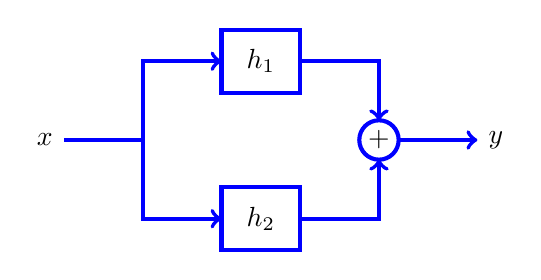
\begin{tikzpicture}[line width = 1.5pt, draw = blue]
			\draw  (0,0) -- (1,0);
			\draw [->] (1,0) -- (1,1) -- (2,1);
			\draw [->] (1,0) -- (1,-1) -- (2,-1);
			\draw (2,1-.4) rectangle (3,1.4) node[pos=.5] {$ h_1 $};
			\draw (2,-1.4) rectangle (3,-1+.4) node[pos=.5] {$ h_2 $};
			\draw [->] (3,1) -- (4,1) -- (4,.25);
			\draw [->] (3,-1) -- (4,-1) -- (4,-.25);
			\draw (4,0) circle [radius=0.25] node {$+$};
			\draw [->] (4.25,0) -- (5.25,0);
			\node[left]at(0,0){$x$};
			\node[right]at(5.25,0){$y$};
			\end{tikzpicture}
		\end{figure}
	
	\column{.05\textwidth}
	\[\equiv\]
	
	
		\column{.45\textwidth}
		\begin{figure}[h!]
			\centering
			\Large
			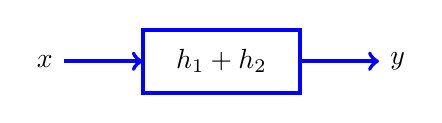
\begin{tikzpicture}[line width = 1.5pt, draw = blue]
			\draw [->] (0,0) -- (1,0);
			\draw (1,-.4) rectangle (3,.4) node[pos=.5] {$ h_1 + h_2$};
			\draw [->] (3,0) -- (4,0);
			\node[left]at(0,0){$x$};
			\node[right]at(4,0){$y$};
			\end{tikzpicture}
		\end{figure}
				
	\end{columns}
\end{frame}

\begin{frame}{The Associative Property}
	\[x*(h_1*h_2) = (x*h_1)*h_2\]
		\begin{columns}
		\column{.45\textwidth}
		\begin{figure}[h!]
			\centering
			\Large
			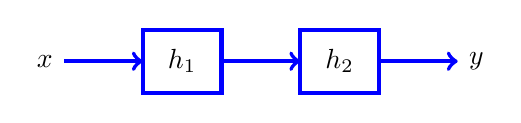
\begin{tikzpicture}[line width = 1.5pt, draw = blue]
			\draw [->] (0,0) -- (1,0);
			\draw (1,-.4) rectangle (2,.4) node[pos=.5] {$ h_1$};
			\draw [->] (2,0) -- (3,0);
			\draw (3,-.4) rectangle (4,.4) node[pos=.5] {$ h_2$};
			\draw [->] (4,0) -- (5,0);
			\node[left]at(0,0){$x$};
			\node[right]at(5,0){$y$};
			\end{tikzpicture}
		\end{figure}
		
		\column{.05\textwidth}
		\[\equiv\]
		
		
		\column{.45\textwidth}
		\begin{figure}[h!]
			\centering
			\Large
			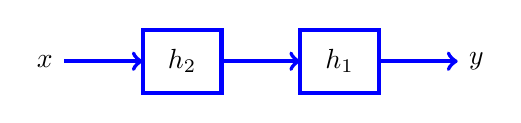
\begin{tikzpicture}[line width = 1.5pt, draw = blue]
			\draw [->] (0,0) -- (1,0);
			\draw (1,-.4) rectangle (2,.4) node[pos=.5] {$ h_2$};
			\draw [->] (2,0) -- (3,0);
			\draw (3,-.4) rectangle (4,.4) node[pos=.5] {$ h_1$};
			\draw [->] (4,0) -- (5,0);
			\node[left]at(0,0){$x$};
			\node[right]at(5,0){$y$};
			\end{tikzpicture}
		\end{figure}
		
	\end{columns}
\[\equiv\]
\centering
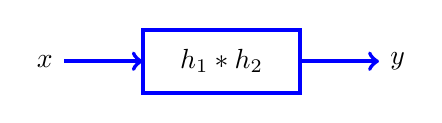
\begin{tikzpicture}[line width = 1.5pt, draw = blue]
	\draw [->] (0,0) -- (1,0);
	\draw (1,-.4) rectangle (3,.4) node[pos=.5] {$ h_1 * h_2$};
	\draw [->] (3,0) -- (4,0);
	\node[left]at(0,0){$x$};
	\node[right]at(4,0){$y$};
\end{tikzpicture}

\end{frame}

\begin{frame}{Memorylessness}
	An LTI system is memoryless if and only if $ h[n] = 0 $ for $ n\neq 0 $, so the impulse response has the form 
	\[h[n] = K\delta[n]\]
	or
	\[h(t) = K\delta(t)\]
	As a result (convolution), a memoryless LTI system has the simple input-output relationship
	\[y = Kx\]
\end{frame}

\begin{frame}{Invertibility}
	An LTI system with impulse response $ h $ is invertible if there exists a signal $ h_i $ such that
	\[h*h_i = \delta\]
			\begin{columns}
		\column{.45\textwidth}
		\begin{figure}[h!]
			\centering
			\Large
			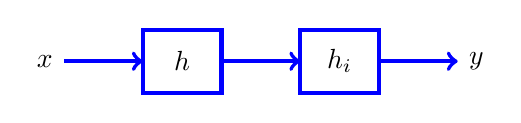
\begin{tikzpicture}[line width = 1.5pt, draw = blue]
			\draw [->] (0,0) -- (1,0);
			\draw (1,-.4) rectangle (2,.4) node[pos=.5] {$ h$};
			\draw [->] (2,0) -- (3,0);
			\draw (3,-.4) rectangle (4,.4) node[pos=.5] {$ h_i$};
			\draw [->] (4,0) -- (5,0);
			\node[left]at(0,0){$x$};
			\node[right]at(5,0){$y$};
			\end{tikzpicture}
		\end{figure}
		
		\column{.05\textwidth}
		\[\equiv\]
		
		
		\column{.45\textwidth}
		\begin{figure}[h!]
			\centering
			\Large
			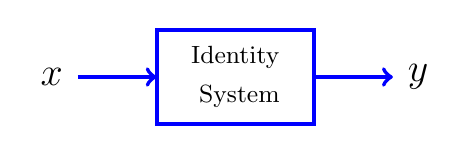
\begin{tikzpicture}[line width = 1.5pt, draw = blue]
			\draw [->] (0,0) -- (1,0);
			\small
			\draw (1,-.6) rectangle (3,.6) node[pos=.5] {$ \begin{aligned}
				\mathrm{Identity}\\
				\mathrm{System}
				\end{aligned} $};
			\Large
			\draw [->] (3,0) -- (4,0);
			\node[left]at(0,0){$x$};
			\node[right]at(4,0){$y$};
			\end{tikzpicture}
		\end{figure}
	\end{columns}
\end{frame}

\begin{frame}{Causality}
	An LTI system with impulse response $ h[n] $ or $ h(t) $ is causal if and only if
	\[h[n] = 0 \quad \text{for } n<0 \]
	or
	\[h(t) = 0 \quad \text{for } t<0 \]
	\vspace{.5cm}
	
	\textbf{Remark: }While causality is a property of systems, it is common terminology to refer to	a signal as being causal if it is zero for $ n < 0 $ or $ t < 0 $.
\end{frame}

\begin{frame}{Stability}
	\begin{block}{Definition}
		A discrete-time signal $ h[n] $ is said to be \textbf{absolutely summable} if 
		\[\sum_{k=-\infty}^{\infty}|h[k]| < \infty\]
	\end{block}
\begin{block}{Definition}
	A continuous-time signal $ h[n] $ is said to be \textbf{absolutely integrable} if 
	\[\int_{-\infty}^{\infty}|h(\tau)|\mathrm{d}\tau < \infty\]
\end{block}

\end{frame}

\begin{frame}{Stability}
	An LTI system is stable if and only if its impulse response is absolutely summable or absolutely integrable.
	
\only<2-5>{	\textbf{Proof($ \Rightarrow $)}:\\
	If $ |x[n]|<B $ for all $ n $, and $ \sum_{k=-\infty}^{\infty}|h[k]|<\infty $:}
\only<2-5>{
	\begin{align*}
		\only<3-5>{ |y[n]| &= \left|\sum_{k=-\infty}^{\infty}h[k]x[n-k]\right|\\}
		\only<4-5>{&\leq\sum_{k=-\infty}^{\infty}|h[k]|\:|x[n-k]|\\ }
		\only<5>{&\leq B\sum_{k=-\infty}^{\infty}|h[k]| < \infty }
	\end{align*}
}
\only<6->{	\textbf{Proof($ \Leftarrow $)}:\\
	If $ \sum_{k=-\infty}^{\infty}|h[k]|=\infty $, we show that there exists a bounded input $ x[n] $ for which the system output grows unbounded.}
	\only<7->{
		\[x[n] = \begin{cases}
		0 & h[-n] = 0\\
		\frac{|h[-n]|}{h[-n]} & h[-n]\neq0
		\end{cases} \quad\Rightarrow\quad |x[n]|\leq 1\]
	}
\only<8>{
\[
	y[0] = \sum_{k=-\infty}^{\infty}x[k]h[-k]
	= \sum_{k=-\infty}^{\infty}|h[-k]| = \infty
 \]
}
\end{frame}


\end{document}